\documentclass{article}
\usepackage{tikz}
\usepackage{tkz-euclide}
\usepackage{pgfplots}

\usetikzlibrary{arrows.meta}
\begin{document}
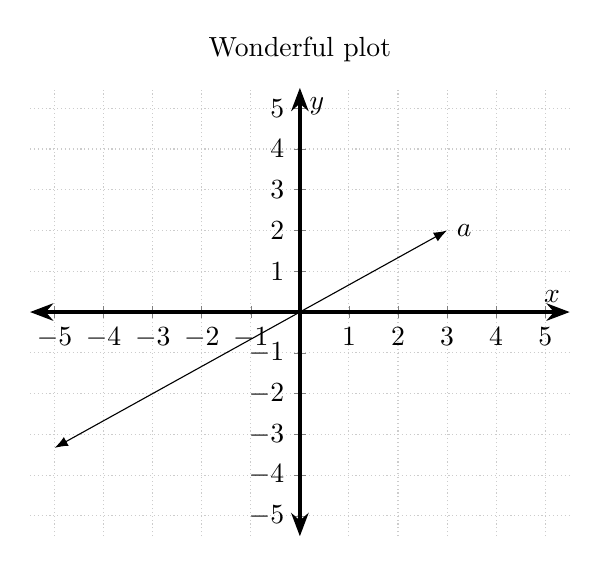
\begin{tikzpicture}
\begin{axis}[
  axis lines=middle,
  axis line style={Stealth-Stealth,very thick},
  xmin=-5.5,xmax=5.5,ymin=-5.5,ymax=5.5,
  xtick distance=1,
  ytick distance=1,
  xlabel=$x$,
  ylabel=$y$,
  title={Wonderful plot},
  grid=major,
  grid style={thin,densely dotted,black!20}]
\addplot [Latex-Latex,domain=-5:3,samples=2] {x*2/3} node[right]{$a$};
\end{axis}
\end{tikzpicture}

\vspace{1cm}

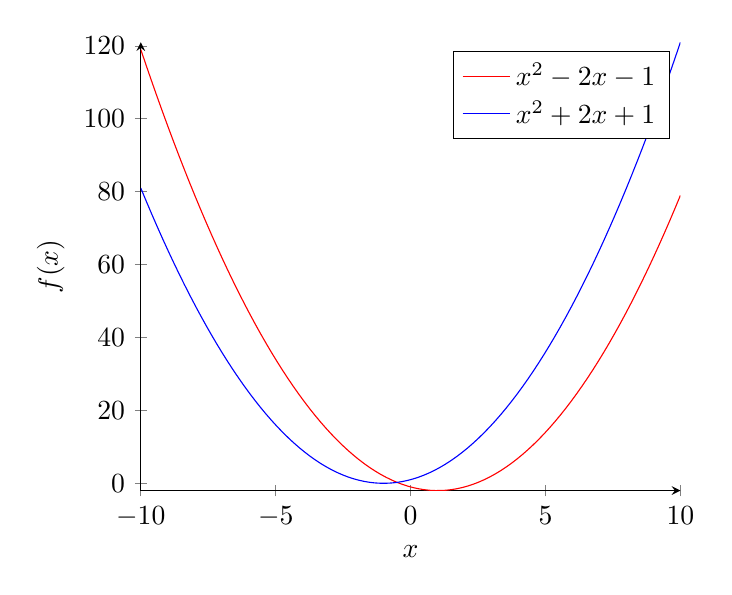
\begin{tikzpicture}
\begin{axis}[
    axis lines = left,
    xlabel = \(x\),
    ylabel = {\(f(x)\)},
]
%Below the red parabola is defined
\addplot [
    domain=-10:10, 
    samples=100, 
    color=red,
]
{x^2 - 2*x - 1};
\addlegendentry{\(x^2 - 2x - 1\)}
%Here the blue parabola is defined
\addplot [
    domain=-10:10, 
    samples=100, 
    color=blue,
    ]
    {x^2 + 2*x + 1};
\addlegendentry{\(x^2 + 2x + 1\)}

\end{axis}
\end{tikzpicture}

\vspace{1cm}

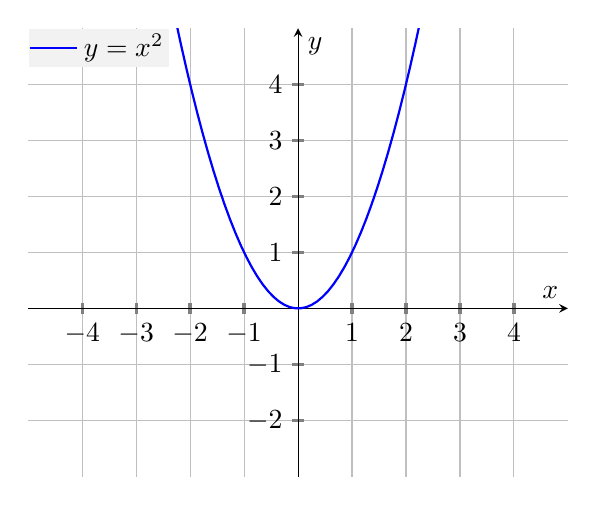
\begin{tikzpicture}
\begin{axis}[
  axis lines=middle,
  grid=major,
  xmin=-5,
  xmax=5,
  ymin=-3,
  ymax=5,
  xlabel=$x$,
  ylabel=$y$,
  xtick={-4,-3,...,4},
  ytick={-2,-1,...,4},
  tick style={very thick},
  legend style={
  at={(rel axis cs:0,1)},
  anchor=north west,draw=none,inner sep=0pt,fill=gray!10}
]
\addplot[blue,thick,samples=100] {x^2};
\addlegendentry{$y=x^2$}
\end{axis}
\end{tikzpicture}

\vspace{1cm}

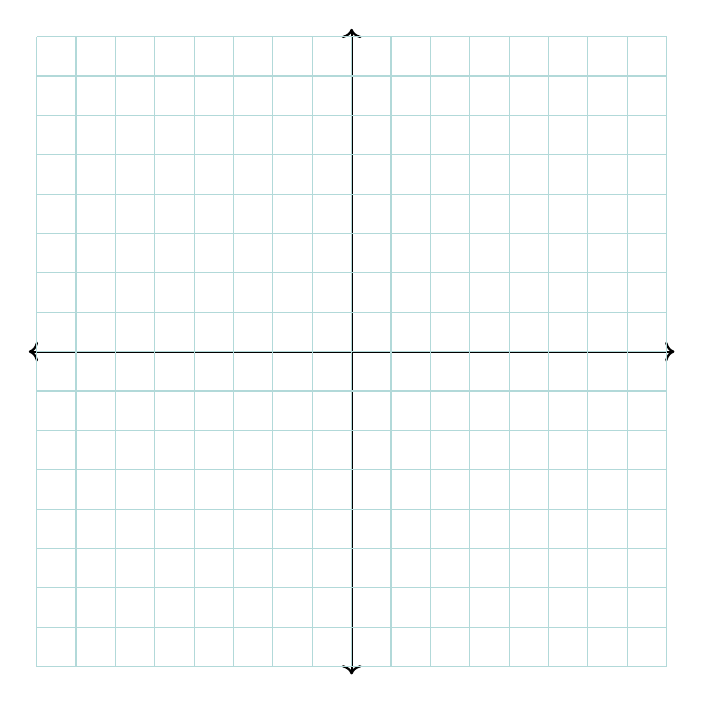
\begin{tikzpicture}
  % axis
  \draw[thick, <->] (0, -4.1) -- (0, 4.1);
  \draw[thick, <->] (-4.1, 0) -- (4.1, 0);

  % grid
  \draw[help lines, step = 0.5cm] (-4, -4) grid (4, 4);
\end{tikzpicture}

\vspace{1cm}

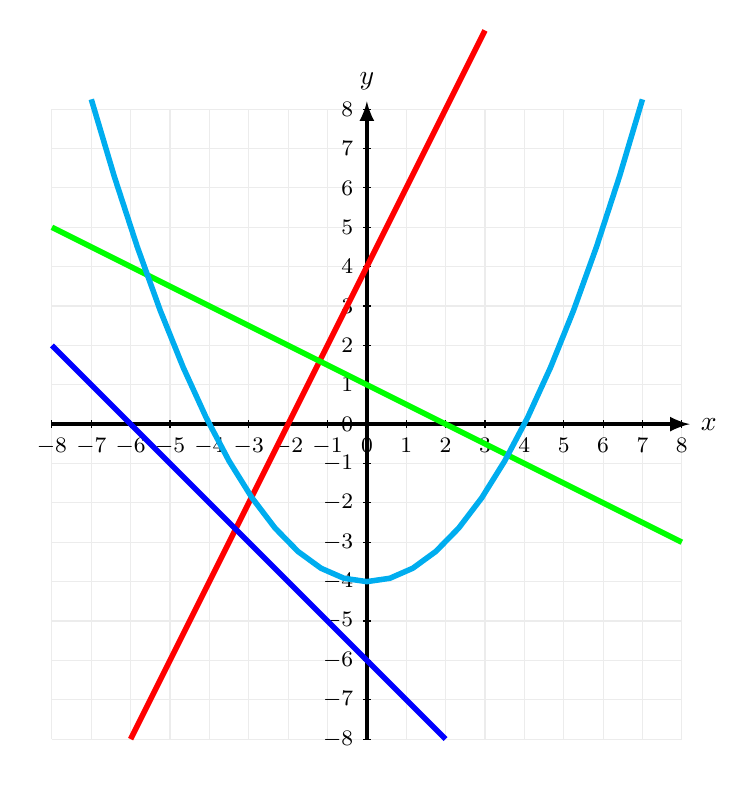
\begin{tikzpicture}[scale=0.50]
        \draw[gray!15,step=1cm] (-8,-8) grid (8,8);    
        \draw[line width=0.5mm, -latex] (-8,0) -- (8.2,0) node[right] {$x$};
        \foreach \x in {-8,...,8} \draw (\x,.1)--(\x,-.1) node[below] {\footnotesize $\x$};
        \draw[line width=0.5mm,  -latex] (0,-8) -- (0,8.2) node[above] {$y$};
        \foreach \y in {-8,...,8} \draw (.1,\y)--(-.1,\y) node[left] {\footnotesize $\y$};
        \draw[red,line width=2pt] plot[domain= -6:3] (\x,{2*\x+4});
        \draw[blue,line width=2pt] plot[domain= -8:2] (\x,{-1*\x-6});
        \draw[green,line width=2pt] plot[domain= -8:8] (\x,{-0.5*\x+1});
        \draw[cyan,line width=2pt] plot[domain= -7:7] (\x,{0.25*\x*\x-4});
\end{tikzpicture}

\vspace{1cm}

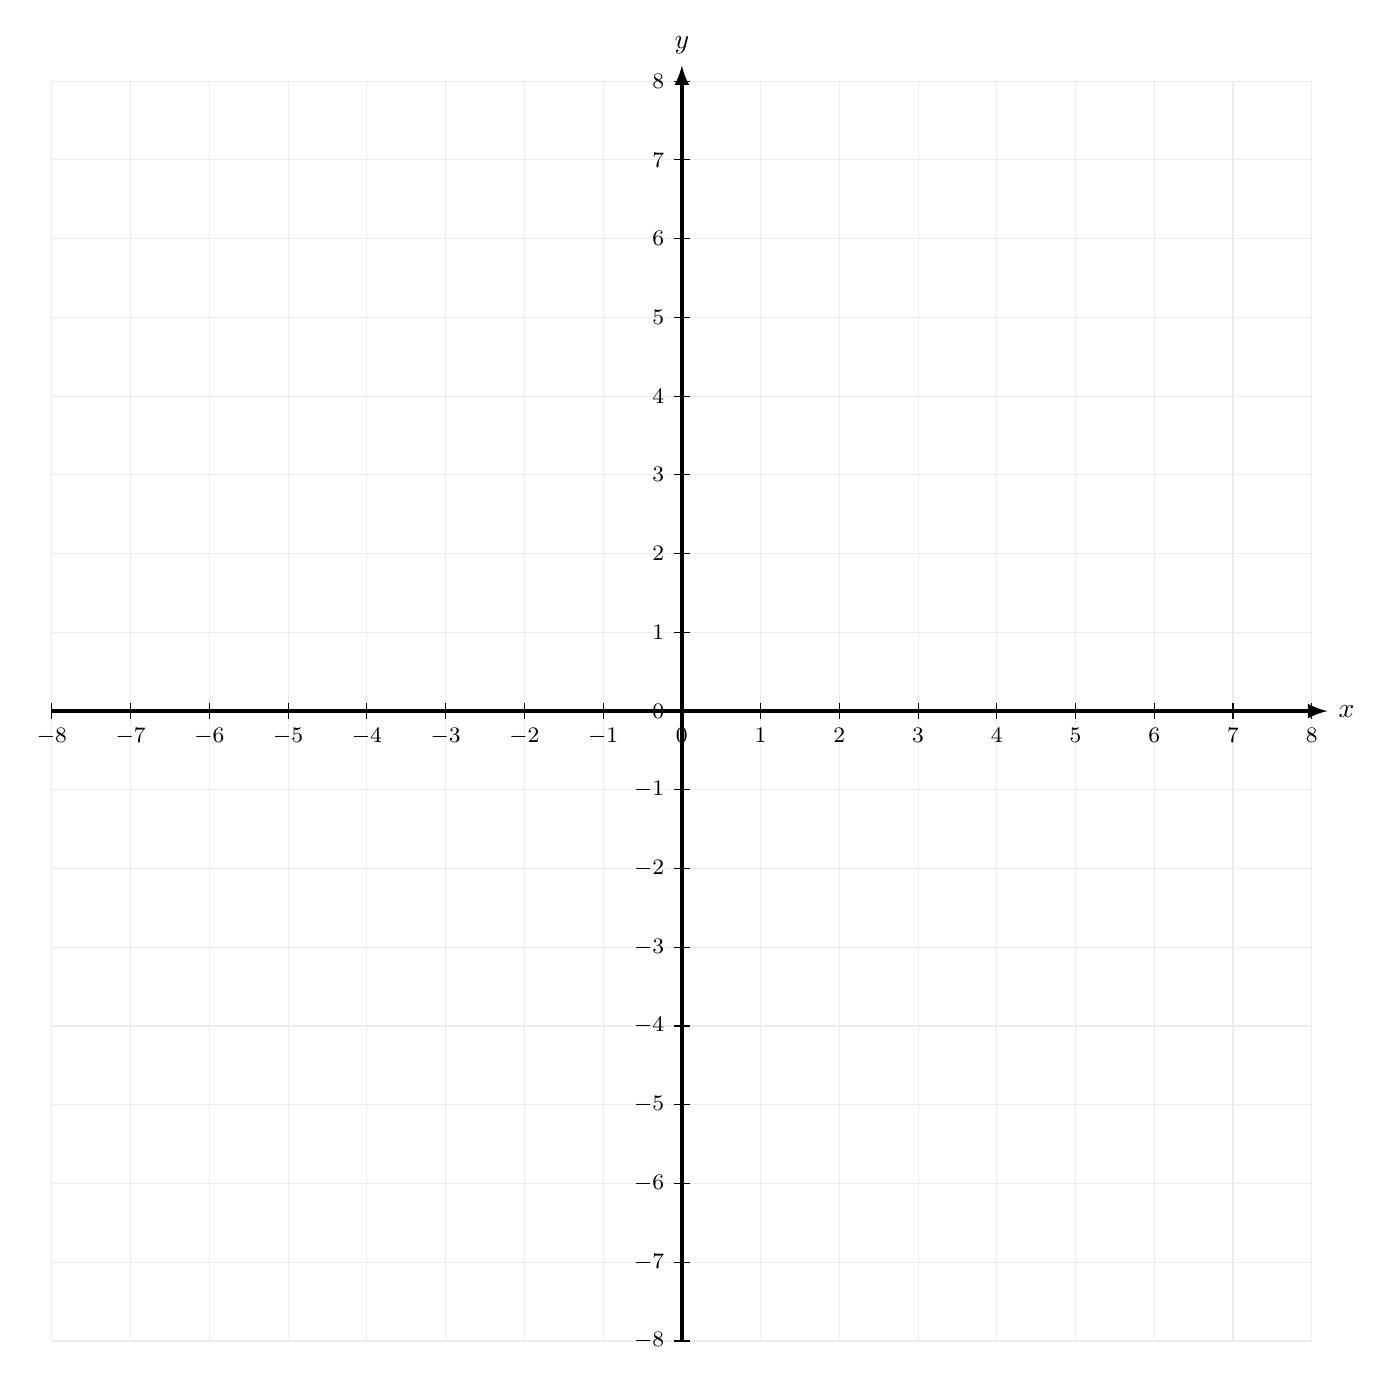
\begin{tikzpicture}
        \draw[gray!15,step=1cm] (-8,-8) grid (8,8);    
        \draw[line width=0.5mm, -latex] (-8,0) -- (8.2,0) node[right] {$x$};
        \foreach \x in {-8,...,8} \draw (\x,.1)--(\x,-.1) node[below] {\footnotesize $\x$};
        \draw[line width=0.5mm,  -latex] (0,-8) -- (0,8.2) node[above] {$y$};
        \foreach \y in {-8,...,8} \draw (.1,\y)--(-.1,\y) node[left] {\footnotesize $\y$};
        
\end{tikzpicture}
\end{document}

